\section{Single Shot Detections}
\begin{frame}{}
    \LARGE Object Detection: \textbf{Single Shot Detections}
\end{frame}

\begin{frame}{Dealing with Scale}
\begin{itemize}
    \item We need to detect objects of many different scales.
    \item How to improve scale invariance of the detector
\end{itemize}

\begin{figure}
\centering
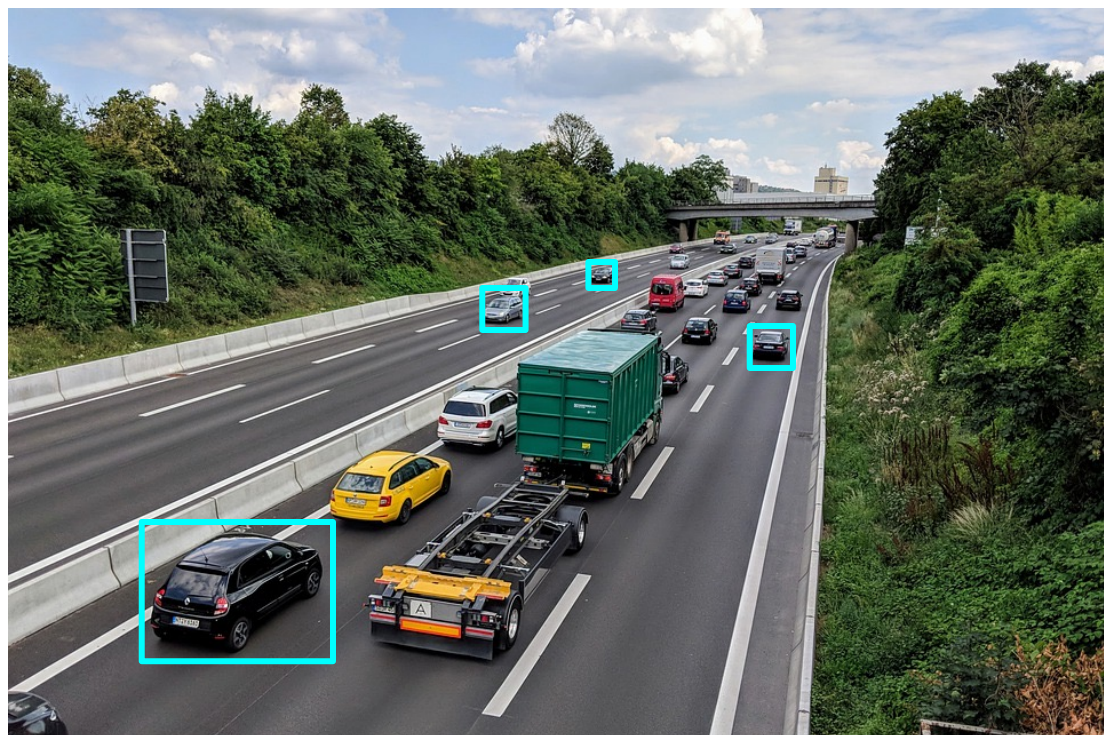
\includegraphics[width=1.0\textwidth,height=0.7\textheight,keepaspectratio]{images/object-detect/scale_1.png}
\end{figure}
    
\end{frame}

\begin{frame}[allowframebreaks]{Dealing with Scale: Image Pyramid}
\begin{figure}
\centering
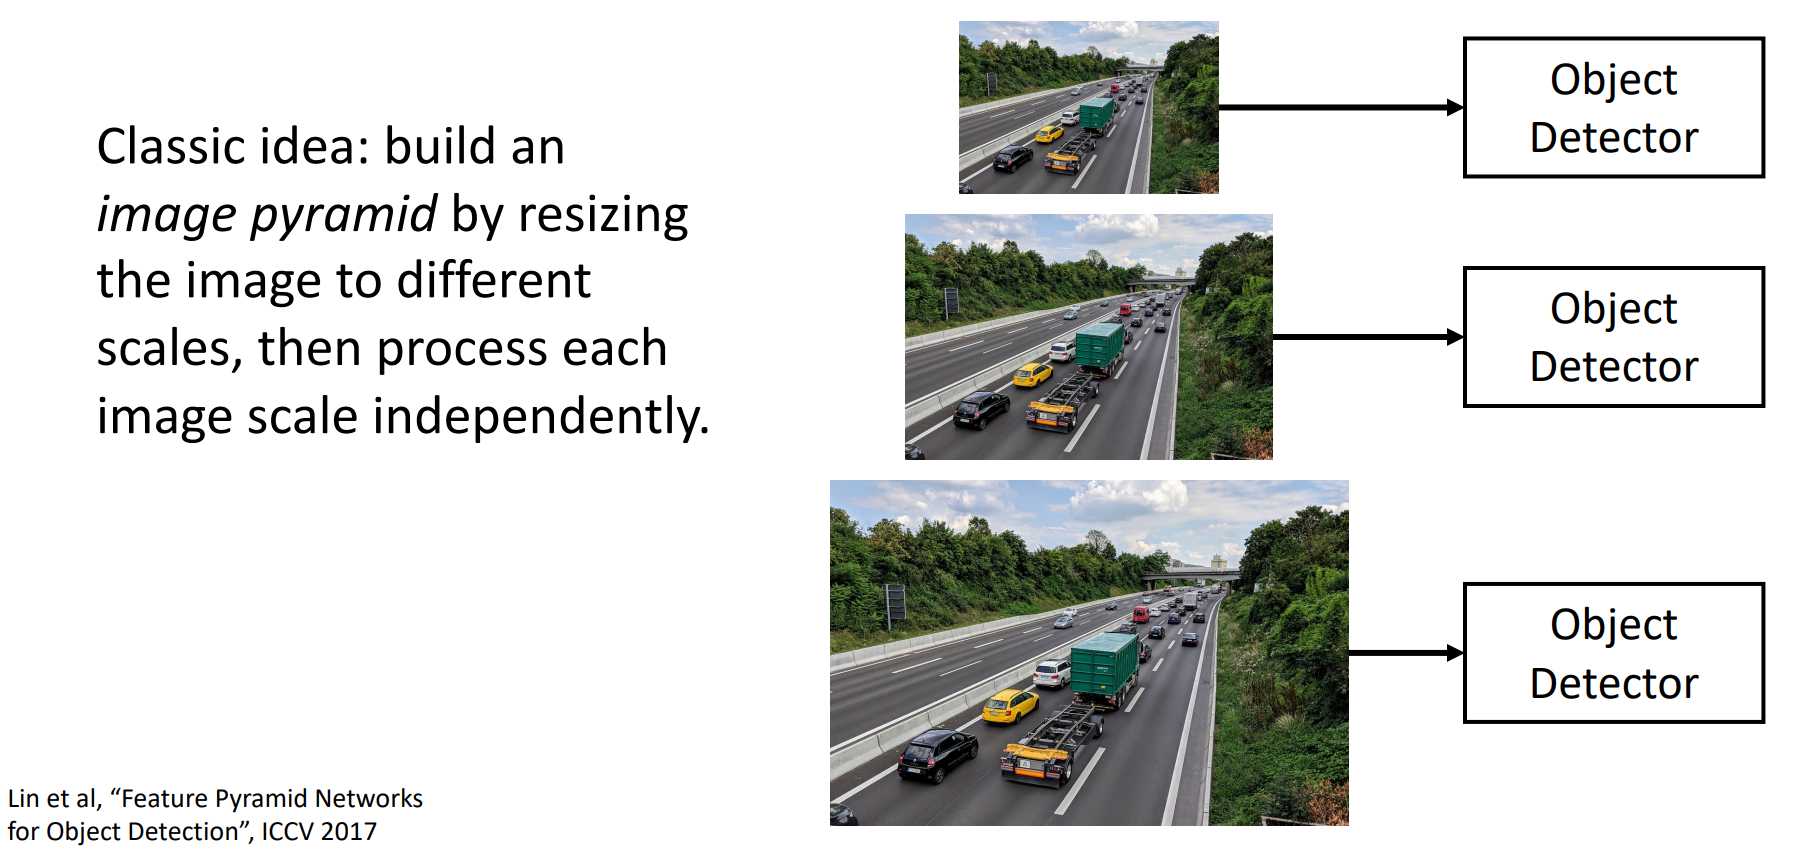
\includegraphics[width=1.0\textwidth,height=1.0\textheight,keepaspectratio]{images/object-detect/scale_2.png}
\end{figure}

\framebreak

\begin{figure}
\centering
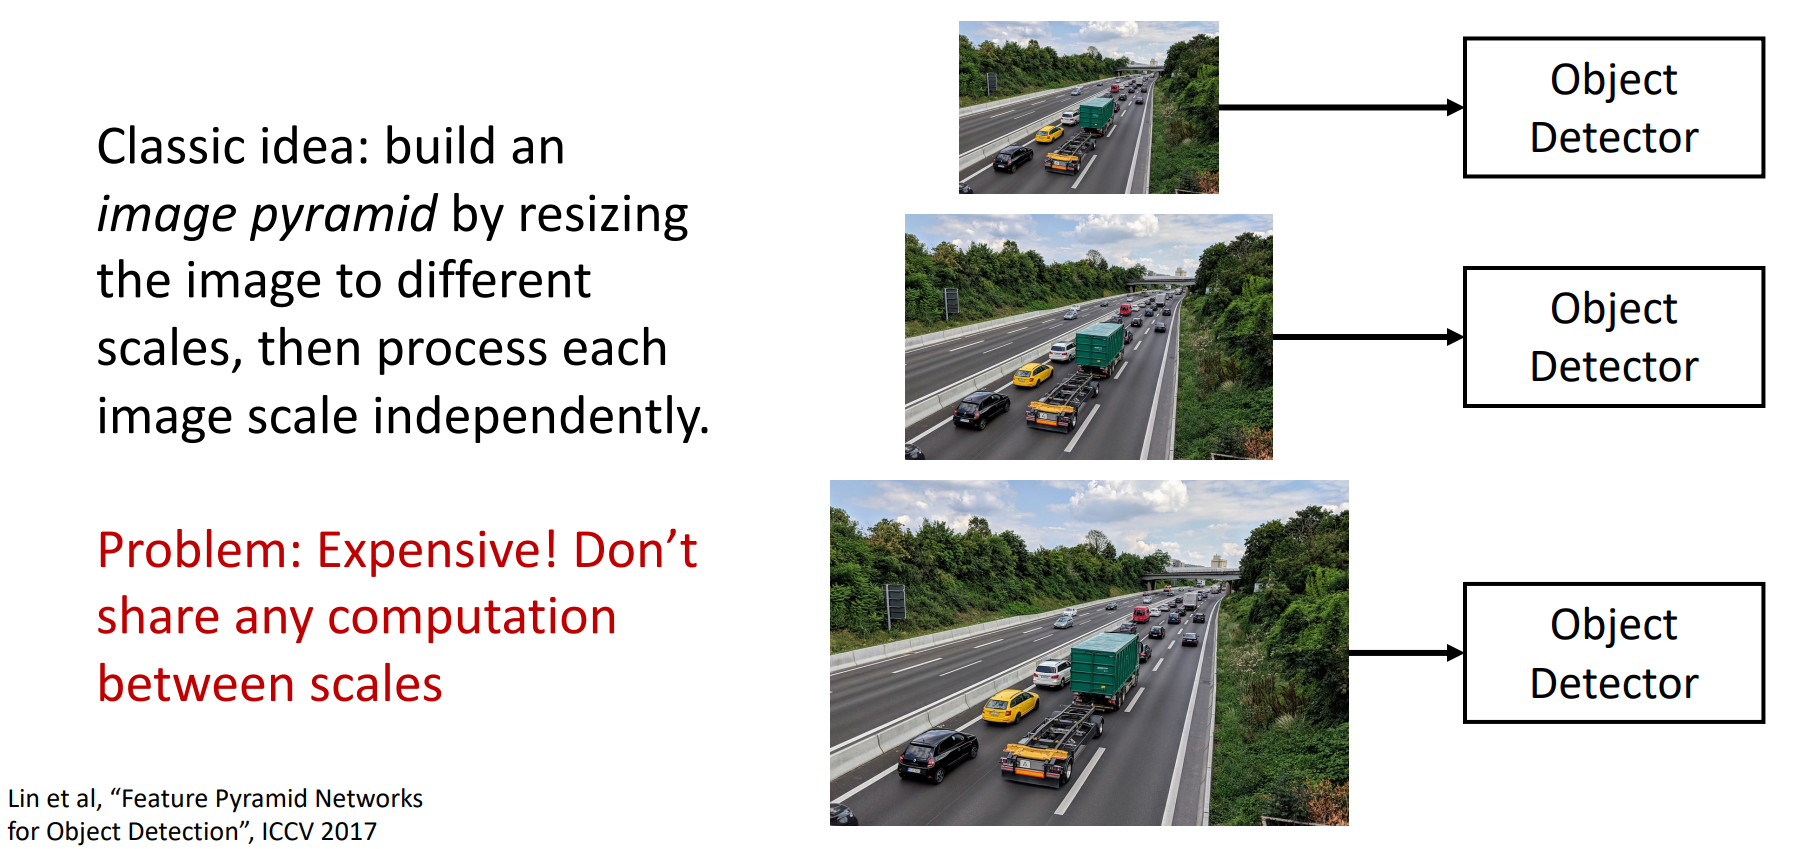
\includegraphics[width=1.0\textwidth,height=1.0\textheight,keepaspectratio]{images/object-detect/scale_3.png}
\end{figure}
    
\end{frame}

\begin{frame}[allowframebreaks]{Dealing with Scale: Image Pyramid}
\begin{figure}
\centering
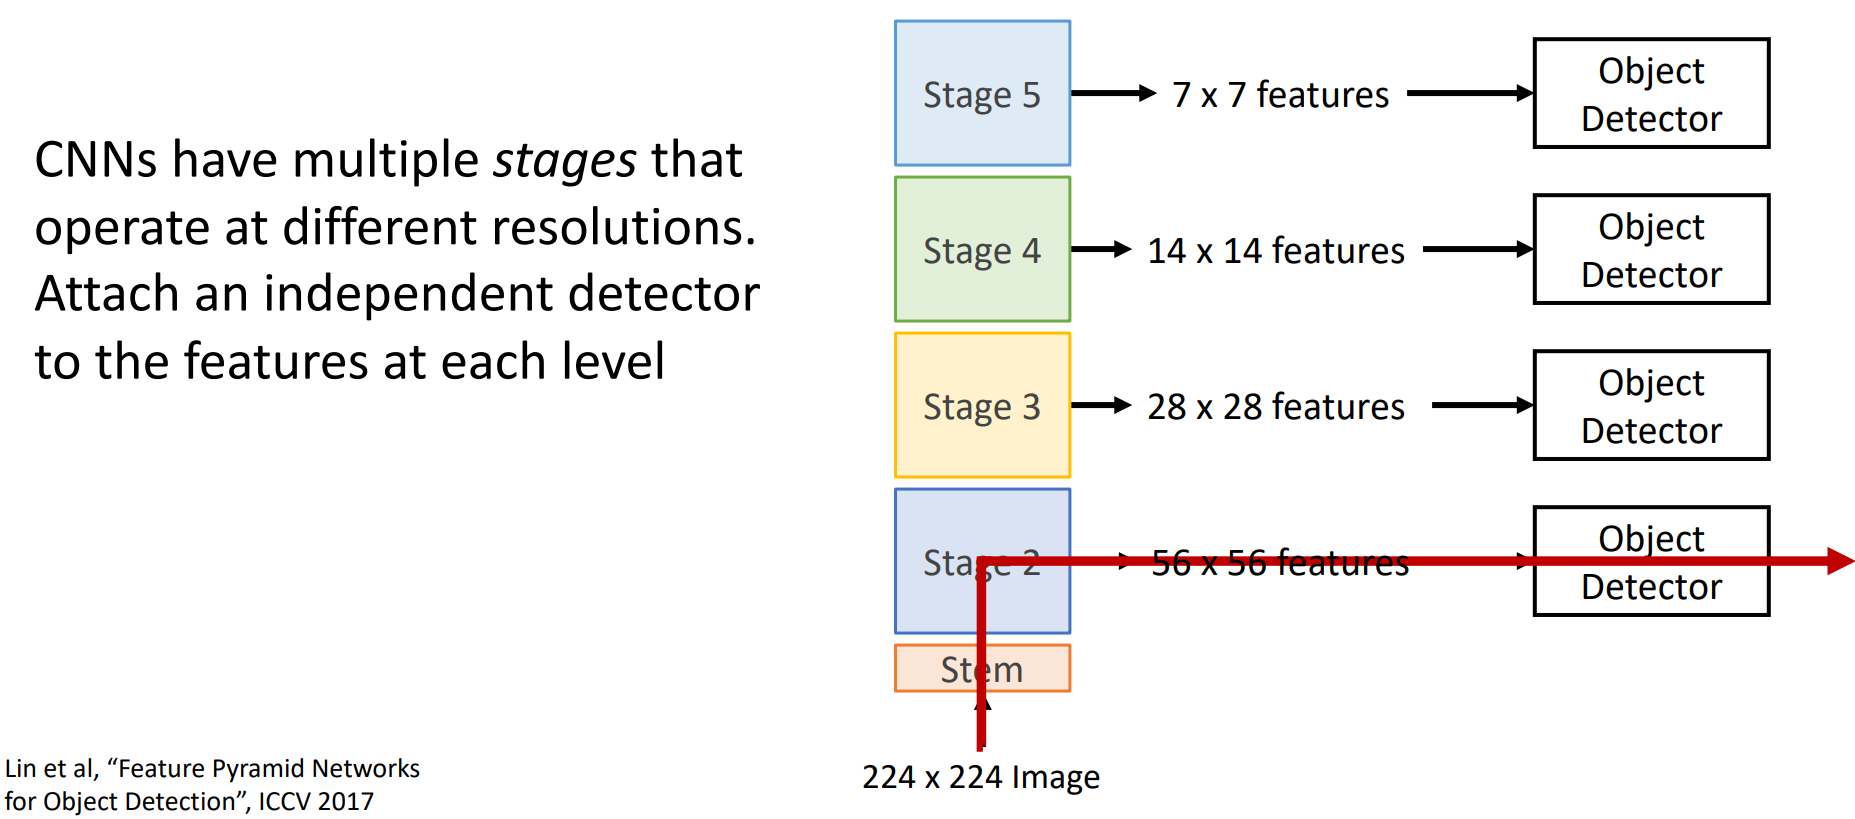
\includegraphics[width=1.0\textwidth,height=1.0\textheight,keepaspectratio]{images/object-detect/scale_4.png}
\end{figure}

\framebreak

\begin{figure}
\centering
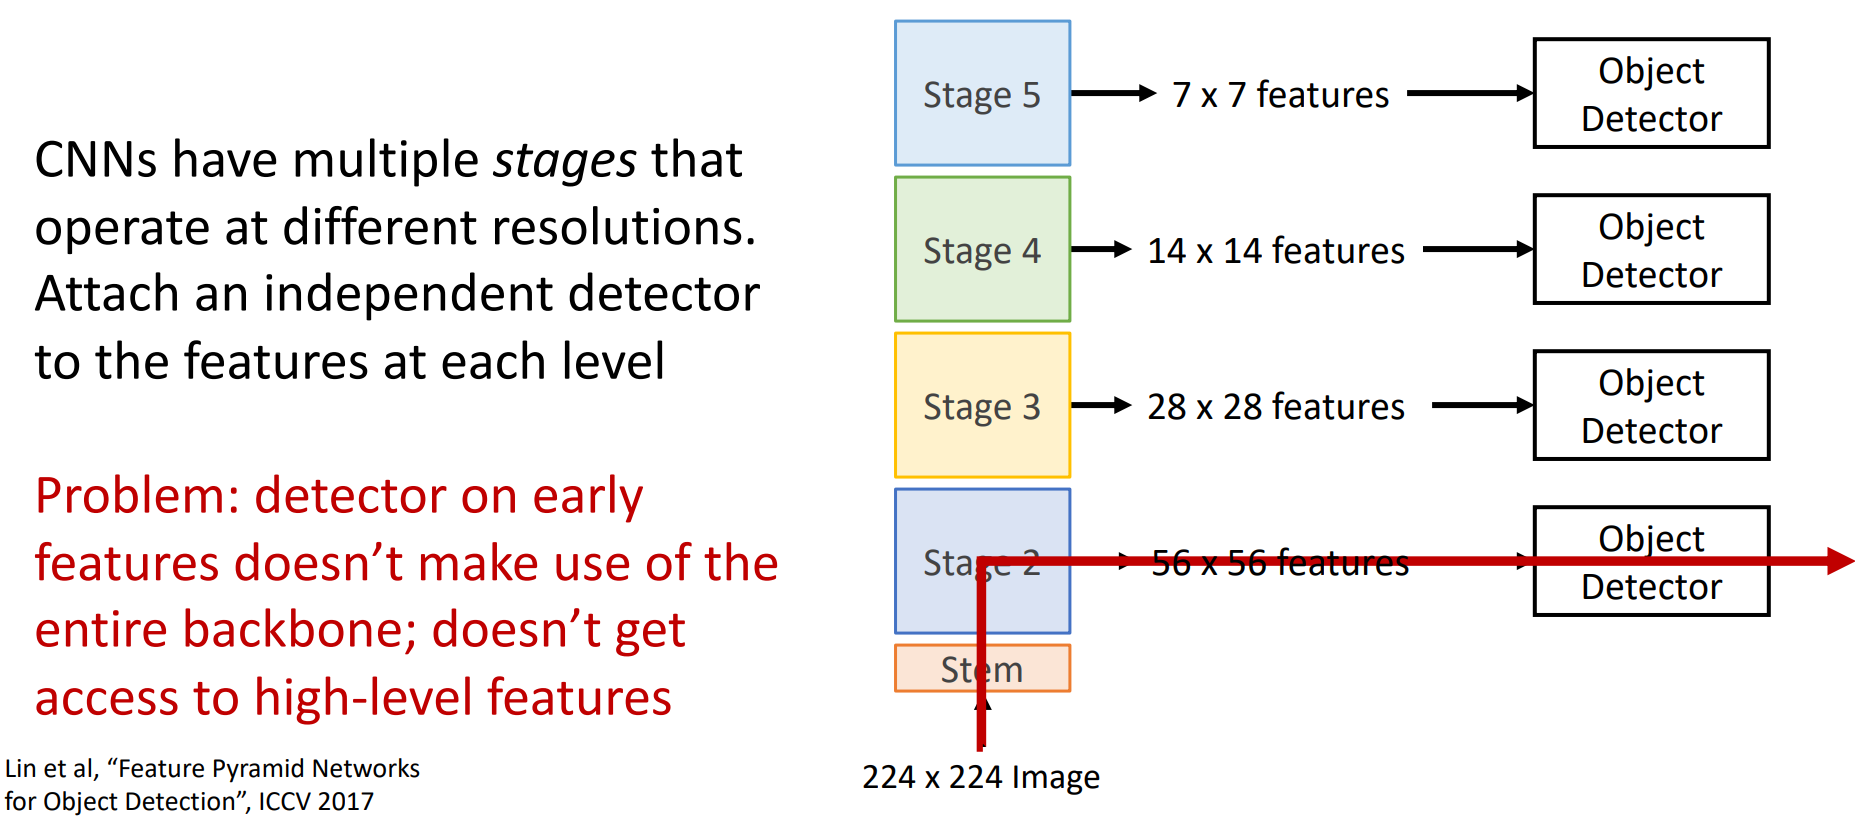
\includegraphics[width=1.0\textwidth,height=1.0\textheight,keepaspectratio]{images/object-detect/scale_5.png}
\end{figure}
    
\end{frame}

\begin{frame}[allowframebreaks]{Dealing with Scale: Feature Pyramid Network}
\begin{figure}
\centering
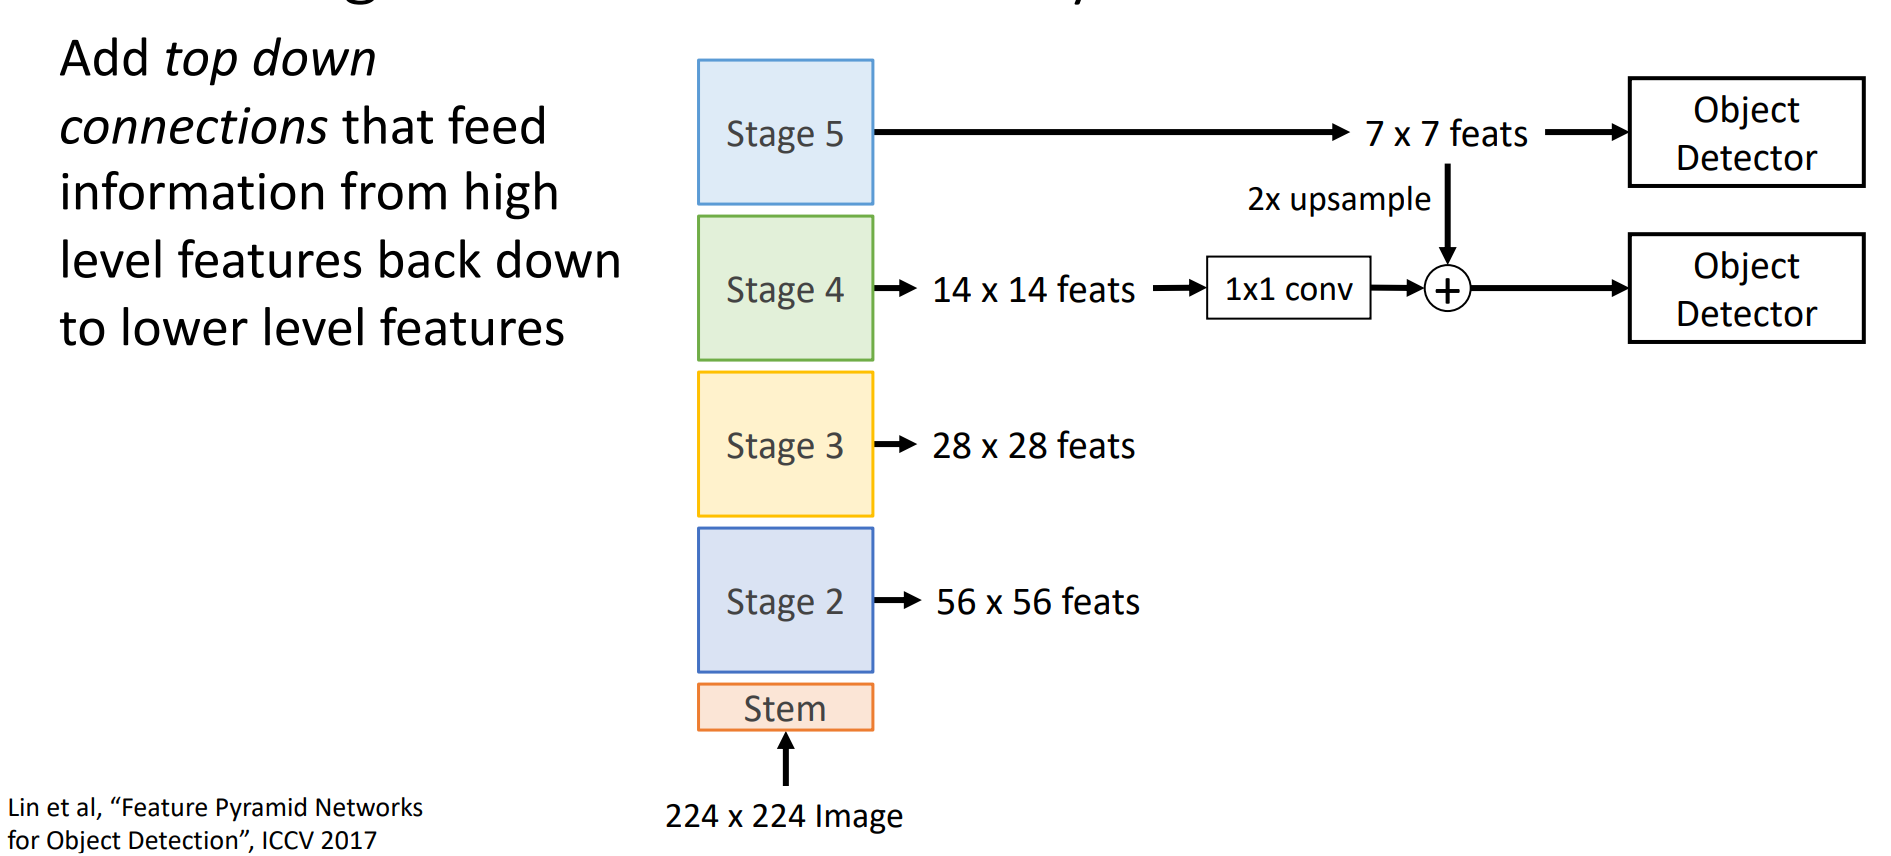
\includegraphics[width=1.0\textwidth,height=1.0\textheight,keepaspectratio]{images/object-detect/scale_6.png}
\end{figure}

\framebreak

\begin{figure}
\centering
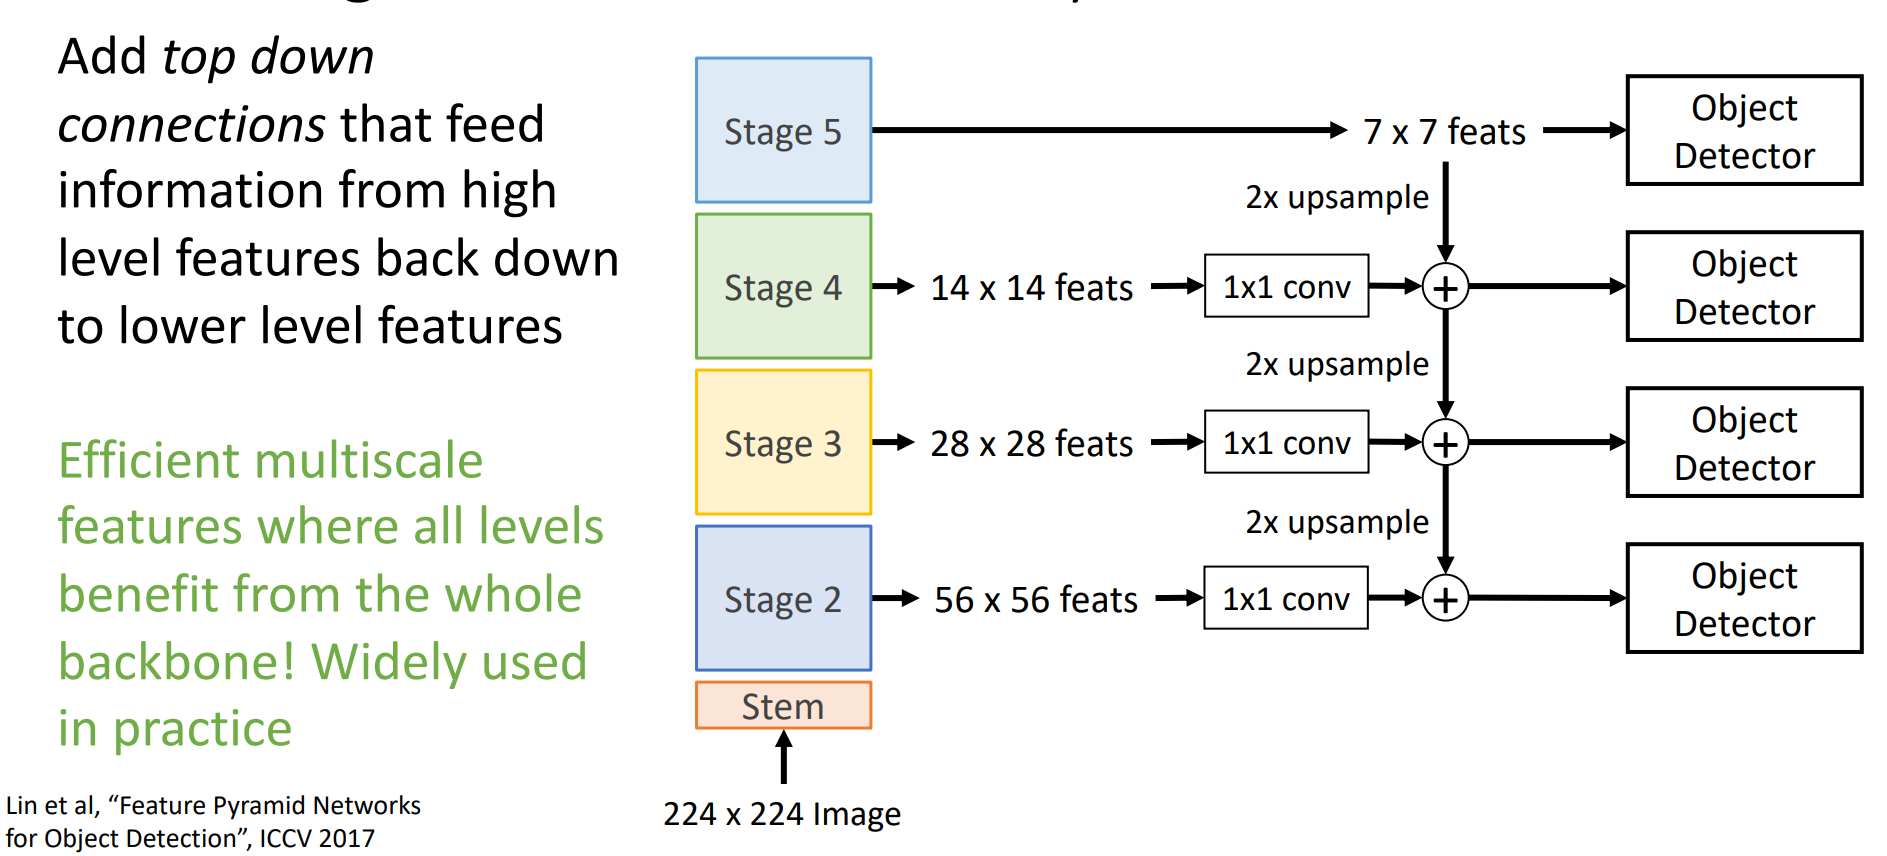
\includegraphics[width=1.0\textwidth,height=1.0\textheight,keepaspectratio]{images/object-detect/scale_7.png}
\end{figure}

\framebreak

\begin{figure}
\centering
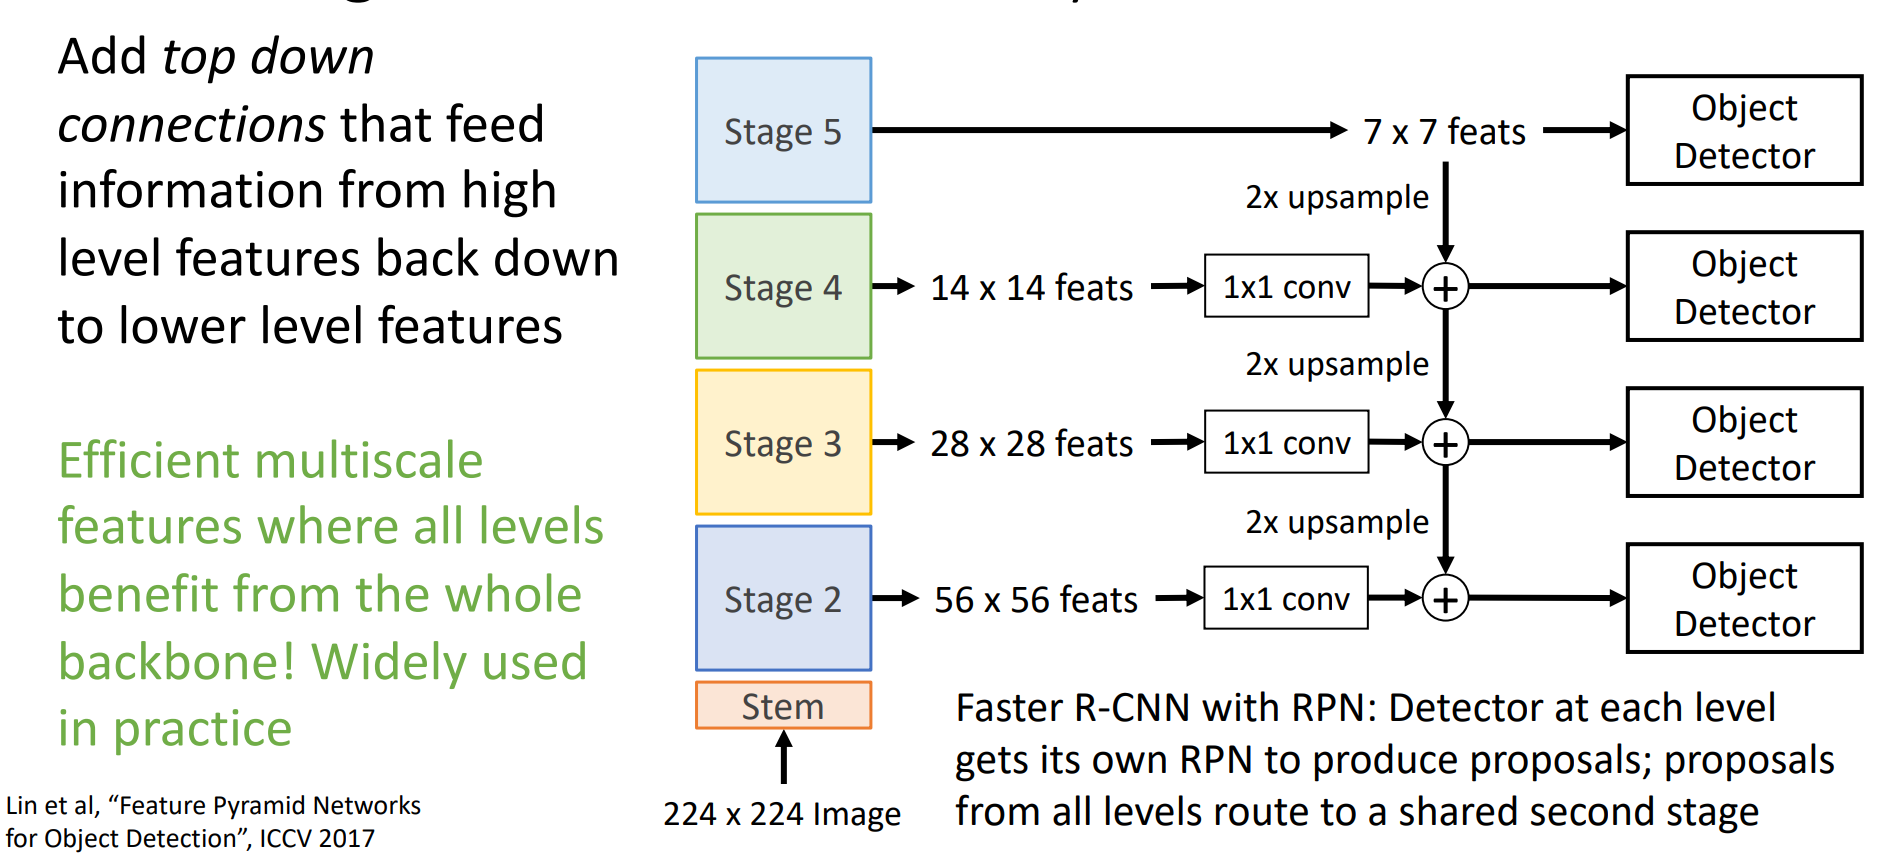
\includegraphics[width=1.0\textwidth,height=1.0\textheight,keepaspectratio]{images/object-detect/scale_8.png}
\end{figure}
    
\end{frame}


\begin{frame}{Overlapping Boxes: Non-Max Suppression (NMS)}
\begin{columns}
    \begin{column}{0.5\textwidth}
    \begin{itemize}
        \item<1-> \textbf{Problem:} Object detectors often output many overlapping detections
        \item<2-> \textbf{Solution:} Post-process raw detections using Non-Max Suppression (NMS)
        \onslide<3->{
        \begin{enumerate}
            \item Select next highest-scoring box
            \item Eliminate lower-scoring boxes 
            \item with IoU $>$ threshold (e.g. 0.7)
            \item If any boxes remain, GOTO 1
        \end{enumerate}
        }
        \item<5-> \textcolor{red}{\textbf{Problem:} NMS may eliminate "good" boxes when objects are highly overlapping… no good solution =( }
    \end{itemize}
    \end{column}
    
    \begin{column}{0.5\textwidth}
    \only<-3>{
    \begin{figure}
    \centering
    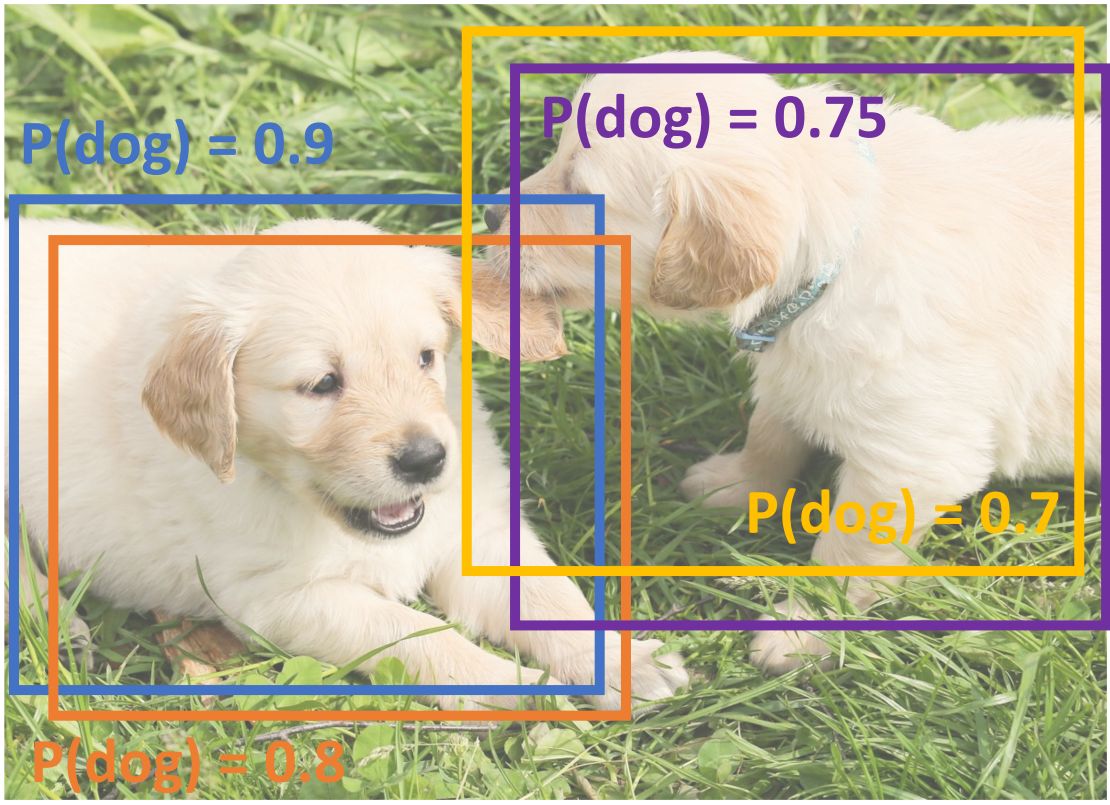
\includegraphics[width=1.0\textwidth,height=1.0\textheight,keepaspectratio]{images/object-detect/nms_1.png}
    \end{figure}
    }

    \only<4>{
    \begin{figure}
    \centering
    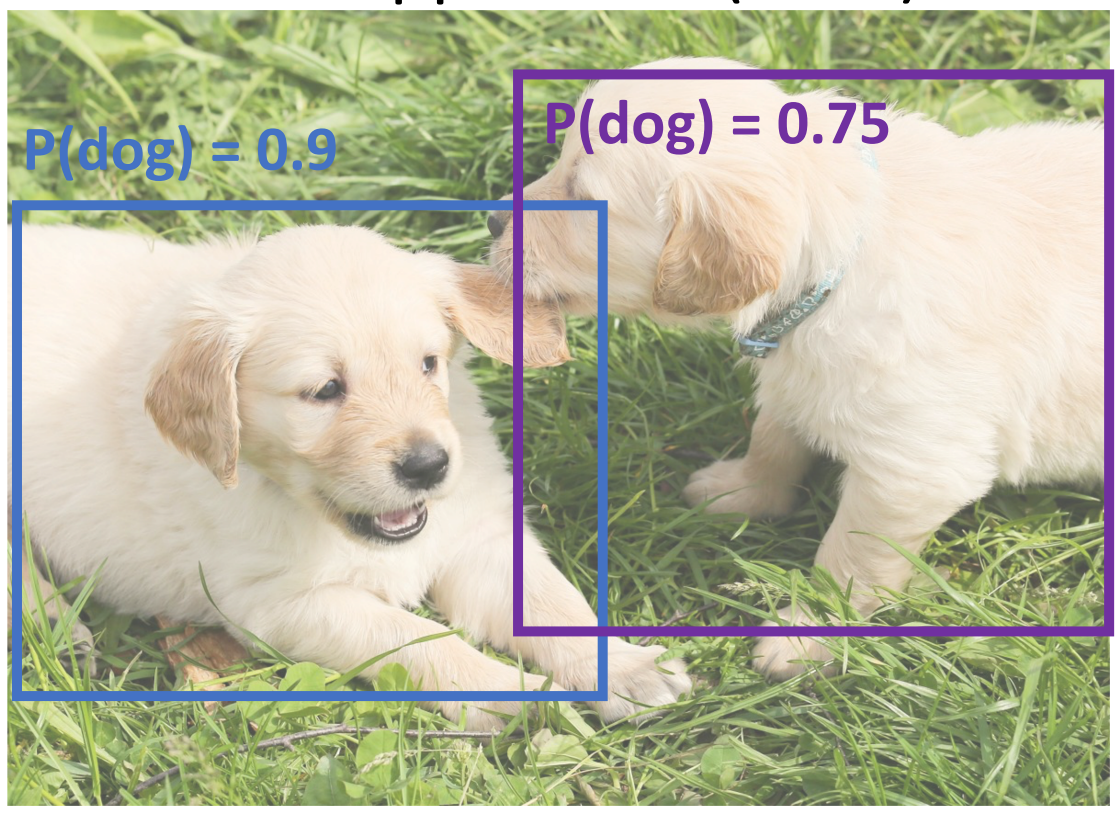
\includegraphics[width=1.0\textwidth,height=1.0\textheight,keepaspectratio]{images/object-detect/nms_2.png}
    \end{figure}
    }

    \only<5>{
    \begin{figure}
    \centering
    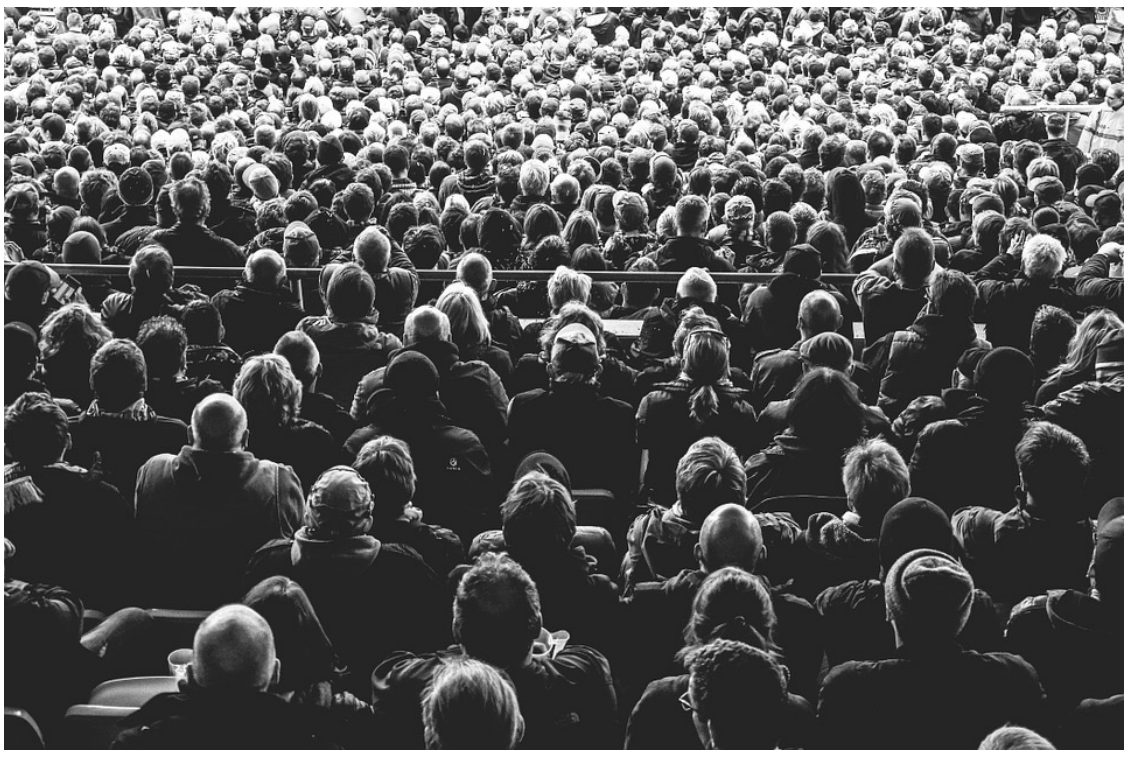
\includegraphics[width=1.0\textwidth,height=1.0\textheight,keepaspectratio]{images/object-detect/nms_3.png}
    \end{figure}
    }
        
    \end{column}
\end{columns}
    
\end{frame}

\begin{frame}{Single Shot Object Detection}
    \begin{figure}
        \centering
        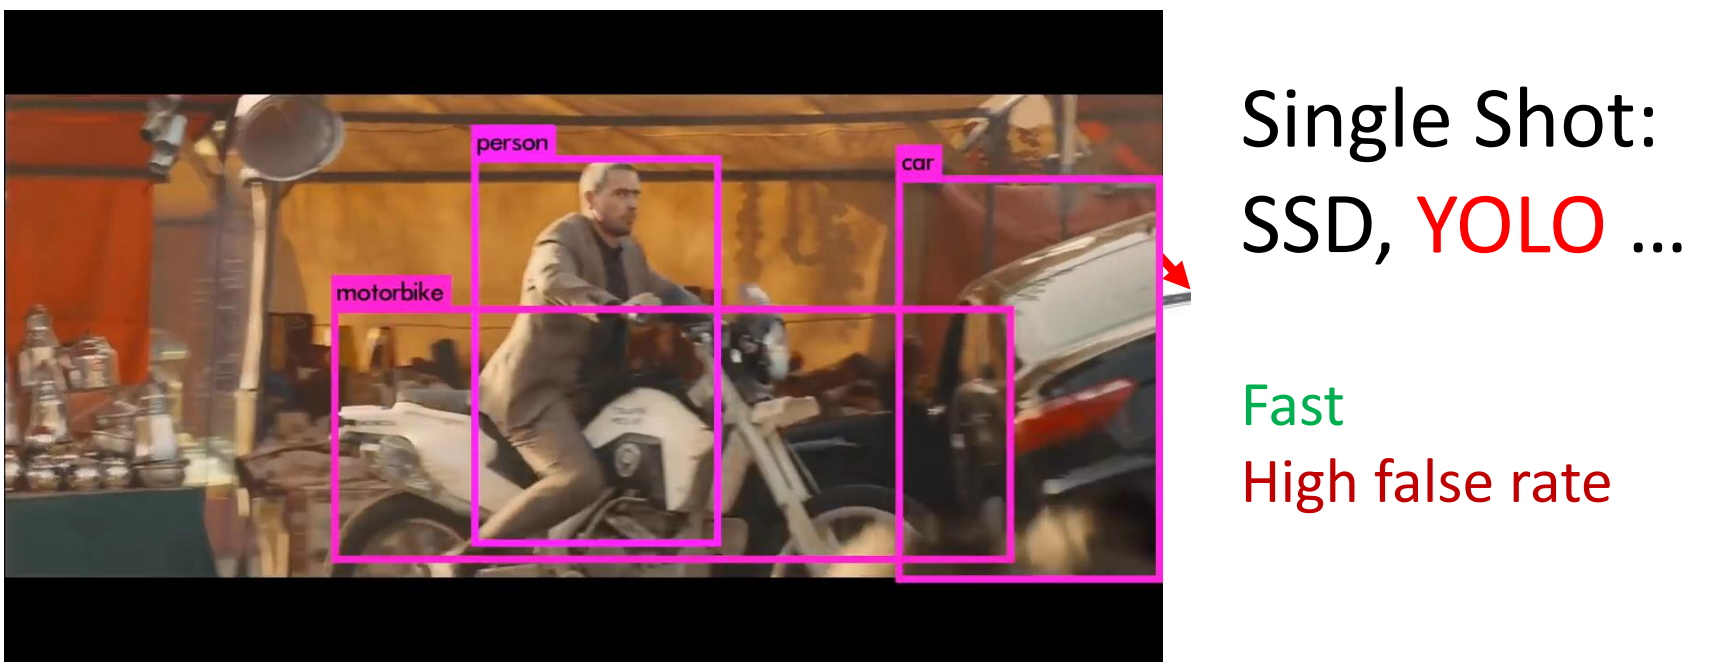
\includegraphics[width=1.0\textwidth,height=1.0\textheight,keepaspectratio]{images/object-detect/yolo_1.png}
    \end{figure}
\end{frame}